% ============================================================
%  Trebuchet (75 %, knock-down) -- step-by-step assembly manual
%  Drawings from steps.py / views.py (built from the cutting geometry)
%  Compile: pdflatex (twice) beside steps/ and view_wedge.pdf
% ============================================================
\documentclass[11pt,a4paper]{article}
\usepackage[T1]{fontenc}
\usepackage[a4paper, top=1.2cm, bottom=1.6cm, left=1.5cm, right=1.5cm]{geometry}
\usepackage{xcolor}
\usepackage{graphicx}
\usepackage{booktabs}
\usepackage{array}
\usepackage{tabularx}
\usepackage{enumitem}
\usepackage{fancyhdr}
\usepackage{amssymb}
\usepackage[protrusion=true,expansion=false]{microtype}

\definecolor{Ink}{HTML}{1A1A1A}
\definecolor{HeadGrey}{HTML}{333333}
\definecolor{RuleGrey}{HTML}{888888}
\definecolor{LineGrey}{HTML}{555555}
\definecolor{WarnBg}{HTML}{F5F5F5}
\definecolor{Badge}{HTML}{C0392B}
\definecolor{NeedBg}{HTML}{F6F1E7}

\setlength{\parindent}{0pt}
\setlength{\parskip}{3pt}
\renewcommand{\arraystretch}{1.15}
\newcolumntype{L}[1]{>{\raggedright\arraybackslash}p{#1}}
\newcolumntype{Y}{>{\raggedright\arraybackslash}X}

\newcommand{\parthead}[2]{%
  \par\vspace{2pt}\noindent
  \colorbox{HeadGrey}{\parbox{\dimexpr\linewidth-2\fboxsep}{\color{white}\large\bfseries #1\hfill\normalsize\mdseries #2}}\par\vspace{4pt}}
\newcommand{\sechead}[1]{%
  \par\vspace{5pt}{\bfseries\large\color{HeadGrey} #1}\\[-4pt]
  {\color{RuleGrey}\rule{\linewidth}{0.8pt}}\par\vspace{1pt}}
\newcommand{\badge}[1]{\colorbox{Badge}{\color{white}\bfseries\large\,#1\,}}
\newcommand{\need}[1]{\par\vspace{3pt}\noindent\colorbox{NeedBg}{\parbox{\dimexpr\linewidth-2\fboxsep}{\footnotesize\textbf{You need:} #1}}\par}
\newcommand{\warn}[1]{\par\vspace{3pt}\noindent\fcolorbox{LineGrey}{WarnBg}{\parbox{\dimexpr\linewidth-2\fboxsep-2\fboxrule}{\footnotesize #1}}\par}

% \step{num}{title}{image}{image width}{text}
\newcommand{\step}[5]{%
  \par\vspace{6pt}\noindent
  \begin{minipage}[t]{#4\linewidth}\vspace{0pt}\centering\includegraphics[width=\linewidth]{#3}\end{minipage}\hfill
  \begin{minipage}[t]{\dimexpr0.97\linewidth-#4\linewidth\relax}\vspace{0pt}
    \badge{#1}\;{\bfseries\large #2}\par\vspace{4pt}\small #5
  \end{minipage}\par\vspace{4pt}{\color{RuleGrey!50}\rule{\linewidth}{0.4pt}}}

\pagestyle{fancy}
\fancyhf{}
\renewcommand{\headrulewidth}{0pt}
\fancyfoot[L]{\footnotesize\color{RuleGrey} Trebuchet (75\,\%, knock-down) \textbullet{} Assembly manual}
\fancyfoot[R]{\footnotesize\color{RuleGrey} Page \thepage}

\begin{document}
\small

{\LARGE\bfseries\color{Ink} Trebuchet assembly manual}\\[2pt]
{\large 75\,\% knock-down build \textbullet{} 4\,kg counterweight \textbullet{} 6\,mm plywood}\\[2pt]
{\color{RuleGrey}\rule{\linewidth}{1.2pt}}

\textbf{Part 1} is done once, by staff or the lab technician: it glues the plywood into two \textbf{side units} and builds the \textbf{arm unit}. Allow two sessions, because the glue needs to dry overnight. \textbf{Part 2} is the setup two students do at the start of every session, in about five minutes and with no tools. \textbf{Part 3} is cocking and launching, and \textbf{Part 4} packs it away. Every item in the list below is used in the step named beside it.

The parts are cut from the files in \texttt{labs/lasercut75} (see the cutting notes there). Side B is the \textbf{mirror image} of side A --- keep the A and B parts separate from the moment they come off the laser.

\sechead{What you need, and where it is used}
{\footnotesize
\begin{tabularx}{\linewidth}{@{}Y L{1.0cm} L{1.9cm} Y L{1.0cm} L{1.9cm}@{}}
\toprule
\textbf{Item} & \textbf{Qty} & \textbf{Used in} & \textbf{Item} & \textbf{Qty} & \textbf{Used in} \\
\midrule
\multicolumn{6}{@{}l}{\textit{Frame}} \\
6\,mm dowel, 30 long & 24 & 2, 3 & M10$\times$40 hex bolts (studs) & 4 & 5 \\
25\,mm wood screws & 40 & 7 (32), 9 (2) & M10 star knobs + spring washers & 4 & Set-up 6 \\
PVA wood glue & --- & 2--9 & 8\,mm clevis pins + R-clips & 4 & Set-up 5 \\
\midrule
\multicolumn{6}{@{}l}{\textit{Arm unit}} \\
Aluminium tube 40$\times$20$\times$1.6, 1055 long & 1 & 10 & 6\,mm aluminium plate 100$\times$40 & 4 & 10 \\
M5$\times$40 bolts + nyloc nuts & 6 & 10 & M12$\times$50 hang bolt, nyloc nut, washers & 1 & 10; Set-up 7 \\
M6 eye bolts + nyloc nuts & 2 & 10 & Hardwood plug 17$\times$37$\times$40 + M6 threaded rod, 60 long (release pin) & 1 & 12 \\
UCP204 pillow blocks (20\,mm bore) & 2 & 11; Set-up 6 & 20\,mm steel axle, 360 long & 1 & 11 \\
20\,mm shaft collars & 2 & 11 & Spacer tube (25\,mm conduit), 112 long & 2 & 11 \\
M6$\times$55 bolt + nyloc nut (locks arm to axle) & 1 & 11 & Sensor + hook-and-loop strap & 1 & 11 \\
Low-stretch braided cord, 3\,mm & 2\,m & 12 & 25\,mm steel ring & 1 & 12 \\
\midrule
\multicolumn{6}{@{}l}{\textit{Each session}} \\
90\,mm PVC pipe, halved, 900 long (trough) & 1 & Set-up 7 & Pegs, or 2 sandbags & --- & Set-up 7 \\
4\,kg sand bag, rated strap cradle + shackle & 1 & Set-up 7 & Safety strap (rated sling + carabiner) & 1 & Set-up 7; Launch \\
Trigger loop: 6\,mm rope, 400 long & 1 & Launch 2 & 10\,mm trigger pin, 60 long + 4\,m pull cord & 1 & Launch 2, 5 \\
Sand-filled beanbags 25--125\,g & 2 each & Launch 3 & & & \\
\midrule
\multicolumn{6}{@{}l}{\textbf{Tools:} clamps, drill + 3, 5, 6, 6.5, 12 and 20\,mm bits, spanners (8, 10, 17, 19\,mm), screwdriver, mallet, hacksaw, file, epoxy.} \\
\bottomrule
\end{tabularx}}

\clearpage
\parthead{Part 1 --- Build once}{staff \textbullet{} two sessions}

\step{1}{Check the parts}{steps/b01_inventory.pdf}{0.55}{%
Lay the parts out by type and count them against the drawing. Keep side~A's parts (engraved A) in one pile and side~B's in another.
\begin{itemize}[itemsep=0pt, leftmargin=1.1em, topsep=2pt]
  \item Every structural part is \textbf{two layers}: one numbered 1, one numbered 2.
  \item The rails come in four pieces per side, two per layer.
  \item \textbf{Deliberate spares:} 8 wedges are cut (6 used, 2 spare); 2 sensor plates (1 used, 1 spare); 6 sling pouches (1 used, 5 spare).
  \item \textbf{Tools, not trebuchet parts:} the test piece, the two arm templates and the two doubler templates. Keep the templates for making a replacement arm.
\end{itemize}}

\step{2}{Glue the A-frames}{steps/b02_aframe.pdf}{0.45}{%
For each side, glue layer~2 to layer~1 so that \textbf{both engraved faces point the same way}: the engraving on layer~1 ends up on the outside.
\begin{enumerate}[itemsep=0pt, leftmargin=1.3em, topsep=2pt]
  \item Spread PVA thinly over layer~2.
  \item Lay layer~1 on top and push a 6\,mm dowel through each of the five holes to line the layers up.
  \item Clamp flat on a bench overnight. Trim the dowels flush.
\end{enumerate}
\need{A1 + A2, B1 + B2, 10 dowels, PVA, clamps.}}

\step{3}{Glue the rails}{steps/b03_rail.pdf}{0.55}{%
Each rail is two layers whose joints fall in different places, so the rail is as strong as one long piece.
\begin{enumerate}[itemsep=0pt, leftmargin=1.3em, topsep=2pt]
  \item Lay layer~1's two pieces end to end.
  \item Glue layer~2's two pieces on top, dowel and clamp.
  \item Check that the \textbf{B}, \textbf{M} and \textbf{F} notches underneath line up through both layers.
\end{enumerate}
\need{rail pieces A1, A2 (and B1, B2), dowels, PVA.}}

\step{4}{Glue the cross members and braces}{steps/b04_pairs.pdf}{0.48}{%
Glue each pair face to face, holes and slots lined up: FRONT 1+2, MIDDLE 1+2, BACK 1+2, brace 1+2 and brace 3+4. Push a pin through the brace holes while the glue sets so they line up.
\need{6 cross member layers, 4 brace layers, PVA.}}

\step{5}{Make the top caps}{steps/b05_caps.pdf}{0.45}{%
Each side has a cap on top that carries the bearing.
\begin{enumerate}[itemsep=0pt, leftmargin=1.3em, topsep=2pt]
  \item Push two M10$\times$40 bolts up through the \textbf{hex pockets} in the lower cap. The heads sit flush and cannot turn.
  \item Glue the upper cap on top, the bolts poking up through it. The bolts are now fixed \textbf{studs}.
\end{enumerate}
\need{2 lower + 2 upper caps, 4 M10$\times$40 bolts, PVA.}}

\step{6}{Fit each A-frame into its rail}{steps/b06_frame_on_rail.pdf}{0.5}{%
Glue in the two notches on top of the rail, then drop the A-frame's \textbf{foot tabs} into them. Engraving faces the same way on frame and rail; ``FRONT'' on both points the same way.
\warn{Side~A's frame goes on side~A's rail. The parts only line up the right way round.}}

\step{7}{Add the gussets}{steps/b07_gussets.pdf}{0.5}{%
Glue and screw a gusset over each foot joint, on \textbf{both faces}: four per side unit. The engraved line on each gusset sits along the top of the rail. Four 25\,mm screws through each gusset.
\need{8 gussets, 32 screws, PVA.}}

\step{8}{Glue the cap on top}{steps/b08_cap_on.pdf}{0.45}{%
Glue the cap over the two tabs on top of the A-frame, stud heads down. Check the studs stand upright.

\textbf{Side unit finished.} Build the other side the same way. From now on, a side unit is never taken apart.}

\step{9}{Fit the trigger}{steps/b09_trigger.pdf}{0.5}{%
\begin{enumerate}[itemsep=0pt, leftmargin=1.3em, topsep=2pt]
  \item Glue the three trigger layers together, the slotted one in the middle, pin holes lined up.
  \item Push their tabs into the trigger base and glue.
  \item Glue the base along the top edge of the \textbf{BACK} cross member, centred, and drive two screws down into the edge.
\end{enumerate}
\need{3 trigger layers, trigger base, BACK cross member, 2 screws.}}

\par\vspace{6pt}\noindent\begin{minipage}{\linewidth}\badge{10}\;{\bfseries\large Prepare the arm}\par\vspace{3pt}
\noindent\includegraphics[width=\linewidth]{steps/b10_arm_drill.pdf}\par
\begin{enumerate}[itemsep=0pt, leftmargin=1.3em, topsep=0pt]
  \item Cut the aluminium tube to \textbf{1052--1055\,mm}; file the ends smooth.
  \item Clamp the \textbf{arm end template} flush with one end on a 40\,mm face. Drill 3\,mm pilots for the hang bolt and the axle, then open them up: 12\,mm and 20\,mm, through both walls.
  \item Mark four doubler plates from the templates, cut them from 6\,mm aluminium, drill them, and bolt one each side over each hole with M5 bolts. Re-drill the 12 and 20\,mm holes through the plates.
  \item With the \textbf{tip template} flush with the other end, drill 6\,mm for the sling eye (on the face that will face the trough when cocked) and, on the opposite face, the trigger eye. Fit both M6 eye bolts.
  \item Fit the M12 hang bolt through its hole, nut finger-tight for now. The counterweight's shackle hangs from it.
\end{enumerate}
\end{minipage}
{\color{RuleGrey!50}\rule{\linewidth}{0.4pt}}

\step{11}{Build the arm unit}{steps/b11_arm_unit.pdf}{0.55}{%
\begin{enumerate}[itemsep=0pt, leftmargin=1.3em, topsep=2pt]
  \item Thread the axle through, in this order: collar, pillow block, spacer, \textbf{arm}, spacer, pillow block, collar.
  \item \textbf{Lock the arm to the axle:} centre the arm, then drill 6.5\,mm down through the arm's two narrow faces and straight through the axle. Fit the M6$\times$55 bolt and nyloc nut. The arm and axle now turn together in the bearings.
  \item Tighten the pillow blocks' grub screws on the axle and lock the collars against them.
  \item Spin the arm: it should turn freely and stay centred.
  \item Strap the sensor plate to the arm 100--150\,mm from the axle and the sensor to the plate.
\end{enumerate}}

\step{12}{Release pin and sling}{steps/b10_arm_drill.pdf}{0.45}{%
\begin{enumerate}[itemsep=0pt, leftmargin=1.3em, topsep=2pt]
  \item \textbf{Release pin:} epoxy the hardwood plug into the arm's tip end. Screw the 60\,mm M6 rod 25\,mm into a pilot hole in the plug, along the line of the arm. Round the end.
  \item \textbf{Sling:} cut two 800\,mm cords. Tie one to the sling eye; tie the steel ring to the end of the other. Thread both through the holes in a pouch so that, pulled straight, the pouch's centre is \textbf{750\,mm} from the tip. Both cords exactly the same length.
\end{enumerate}
This \textbf{arm unit} stays assembled from now on, sling attached, so the release stays tuned.
\need{plug, M6 rod, epoxy, 2\,m cord, steel ring, 1 pouch.}}


\newpage
\parthead{Part 2 --- Set up}{two students \textbullet{} about 5 minutes \textbullet{} no tools}

\step{1}{Lay out the cross members}{steps/s01_crossmembers.pdf}{0.5}{%
On flat ground, lay the three cross members parallel, on their long edges, about where the B, M and F letters are on the rails:
\begin{itemize}[itemsep=0pt, leftmargin=1.1em, topsep=2pt]
  \item \textbf{BACK} --- the one with the trigger on top;
  \item \textbf{MIDDLE} --- the longest;
  \item \textbf{FRONT} --- towards the target.
\end{itemize}}

\step{2}{Lower side unit A}{steps/s02_side_A.pdf}{0.5}{%
Two people, one at each end. Hold side unit~A upright, engraving facing \textbf{out}, and lower it so the notches under its rail drop over the three cross members.}

\step{3}{Lower side unit B}{steps/s03_side_B.pdf}{0.5}{%
Do the same with side unit~B on the other end of the cross members, engraving facing out. The shoulders of the cross members stop the two sides coming any closer.}

\step{4}{Wedge the cross members}{steps/s04_wedges.pdf}{0.5}{%
Push a wedge through each of the six wedge holes, just outside each rail, \textbf{thin end first}. Tap it in with the heel of your hand (or a mallet) until it is firm. The wedge pulls the cross member's shoulder tight against the rail.
\begin{center}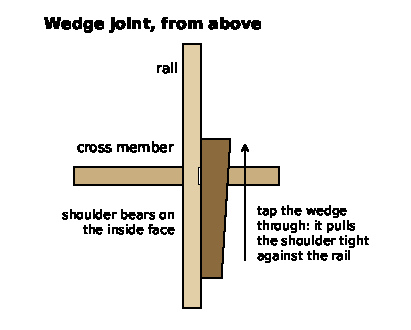
\includegraphics[width=0.8\linewidth]{view_wedge.pdf}\end{center}}

\step{5}{Fit the braces}{steps/s05_braces.pdf}{0.5}{%
For each side:
\begin{enumerate}[itemsep=0pt, leftmargin=1.3em, topsep=2pt]
  \item Push the brace's top tab through the slot in the crossbar, from the outside.
  \item Put a clevis pin through the tab on the inside, and an R-clip through the pin.
  \item Pin the brace's bottom end to the end of the MIDDLE cross member, with an R-clip.
\end{enumerate}
\need{2 braces, 4 clevis pins, 4 R-clips.}}

\step{6}{Fit the arm unit}{steps/s06_arm.pdf}{0.5}{%
Two people. Lift the arm unit, long end up, and lower the pillow blocks over the two studs on each side cap. Spin a star knob down onto each stud: finger tight, then a quarter turn more.
\warn{The arm is drawn short here. The real arm is 750\,mm above the axle: keep clear of its top end.}}

\step{7}{Trough, base and bag}{steps/s07_ready.pdf}{0.5}{%
\begin{enumerate}[itemsep=0pt, leftmargin=1.3em, topsep=2pt]
  \item Lay the trough along the middle of the cross members, from the back cross member to beyond the front one.
  \item Peg the base down, or lay a sandbag on each rail.
  \item With the arm hanging at rest and the \textbf{safety strap on}, clip the 4\,kg bag's strap cradle to the hang bolt with the shackle. Two people for anything over 10\,kg; one is enough for 4\,kg.
\end{enumerate}}

\noindent\begin{minipage}{\linewidth}
\sechead{\badge{8}\; Check before every launch session}
\begin{minipage}[t]{0.49\linewidth}
\begin{itemize}[itemsep=1pt, leftmargin=1.3em, topsep=1pt, label=$\square$]
  \item All six wedges firm
  \item All four star knobs tight
  \item Four brace pins in, R-clips through
  \item The arm turns a full circle by hand without touching anything
\end{itemize}
\end{minipage}\hfill
\begin{minipage}[t]{0.49\linewidth}
\begin{itemize}[itemsep=1pt, leftmargin=1.3em, topsep=1pt, label=$\square$]
  \item The bag clears the trough at the bottom of its swing
  \item Sling cords not frayed; release ring not bent
  \item Base pegged or sandbagged
  \item Exclusion zone and range marked out (Build Guide, page 7)
\end{itemize}
\end{minipage}
\end{minipage}

\clearpage
\parthead{Part 3 --- Cock and launch}{teacher supervises every launch}

\noindent\begin{minipage}[t]{0.56\linewidth}\vspace{0pt}\includegraphics[width=\linewidth]{steps/s08_cocked.pdf}\end{minipage}\hfill
\begin{minipage}[t]{0.42\linewidth}\vspace{0pt}\small
\begin{enumerate}[itemsep=2pt, leftmargin=1.4em, topsep=0pt]
  \item \textbf{Safety strap on.} Everyone except the loader and the operator stands behind the line.
  \item \textbf{Cock it.} Pull the tip of the arm down to the back; the bag rises. Drop the \textbf{trigger loop} (tied to the trigger eye) into the slot in the trigger block and push the \textbf{trigger pin} through the block and the loop. Tie the \textbf{pull cord} to the pin.
  \item \textbf{Load it.} Lay the sling along the trough, beanbag in the pouch, and drop the ring over the release pin.
  \item The teacher checks the range and calls \textbf{``Range clear''}.
  \item Take the safety strap off. The operator stands to the side, behind the line, calls \textbf{``Firing''} and pulls the cord.
  \item Wait until the arm has \textbf{completely stopped}. Safety strap back on before anyone goes near it. Retrieve the beanbag on the teacher's \textbf{``All clear''}.
\end{enumerate}
\end{minipage}

\warn{\textbf{First time only:} commission and tune it as in the Build Guide (page~6): first with no counterweight, then with the 4\,kg bag and no beanbag, then with a beanbag. Once tuned, don't adjust the release pin or the sling again.}

\parthead{Part 4 --- Pack down}{about 3 minutes}
\begin{enumerate}[itemsep=1pt, leftmargin=1.5em, topsep=1pt]
  \item \textbf{Bag off first}, with the arm at rest and the safety strap on.
  \item Star knobs off. Two people lift the arm unit off in one piece. Store it flat with the sling still attached --- it stays tuned.
  \item Pull the brace pins; remove the braces.
  \item Knock the six wedges out (tap the thin end); keep them with the pins and knobs.
  \item Lift side unit~B off the cross members, then side unit~A.
\end{enumerate}
\textbf{Store together:} 2 side units, 3 cross members, 2 braces, the arm unit, the trough, and a box holding: 6 wedges + 2 spares, 4 clevis pins and R-clips, 4 star knobs, the strap cradle and shackle, the safety strap, the trigger loop, trigger pin and pull cord, the sensor and its strap, the spare sensor plate and pouches, and the beanbags.

\end{document}
